%--------------------------------------------------
% CPSC 202: Mathematical Tools for Computer Science
% Yale University
%
% Template for Homework Assignments
% by Yiding Hao
%--------------------------------------------------
\documentclass{cpsc202}

% Please put your information here.
\myname{Chura Quispe, Victor Miguel}
\myprofessor{Marc Masias}
\mysources{Your Sources}
\hwnumber{0}
\lstset{basicstyle=\ttfamily}

% \singlesided % Uncomment to print single-sided.
\graphicspath{{./media/}}
% Start typing your solution here.
\begin{document}

    \centerline{\Large\textbf{Deep Learning Project 1: Image Classification}}

    Objective of the document: Details about the process of implementing algorithms for image classification.

    \large\textbf{Part I: Models from scratch}

    The idea behind iterating over the model's complexity and hyperparameters is to gain insight into the complexity of the problem.
    If a simple model can solve the problem, the iterations should focus on tuning hyperparameters; otherwise, the focus should be on finding the proper model structure.

    After various iterations I will comment three.
    \begin{enumerate}
        \item \textbf{The simple one}: No resizing was applied (although I initially resized the images to 32x32 in the code, which was unnecessary).
        This model consists of only two chains of operations, such as \lstinline|self.pool1(self.relu1(self.conv1(x)))|, followed by a final affine linear transformation like \lstinline|nn.Linear(128, 10)|.
        This approach provided the insight that the model learns quite easily, reaching an accuracy of up to 80\%.
        Based on this, I decided to increase the model's complexity and reduce the learning rate.

        \item \textbf{The complex one}: In this iteration, I maintained the original image size but increased the complexity of each layer and added an extra layer, making it three in total.
        Each layer follows the structure \lstinline|self.pool1(self.bn1(self.relu1(self.conv1(x))))|, with a final affine linear transformation like \lstinline|nn.Linear(512, 10)|.
        However, this approach resulted in a model that was too complex to effectively learn from the data.

        \item \textbf{The medium one}: For this iteration, I used a larger image size of 64x64, added an extra layer, and modified the order of operations within each layer.
        This new model performed better than the previous ones, but its learning stopped after approximately 30 epochs.
    \end{enumerate}

    \begin{figure}[h]
        \caption{Train and Validation / Loss and Accuracy}
        \centering
        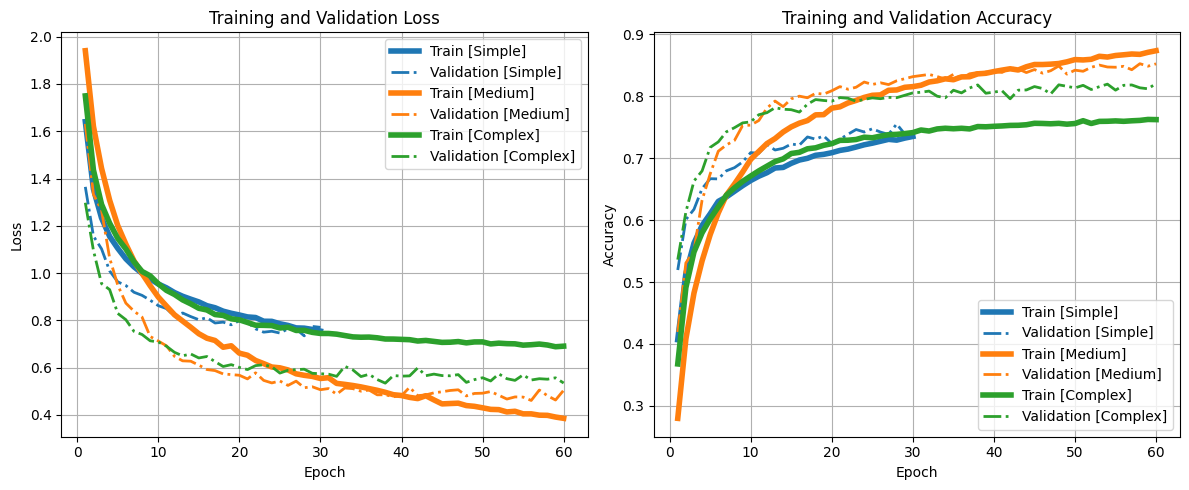
\includegraphics[width=0.9\textwidth]{training_metrics_scratch_01}
        \label{fig:training_metrics_scratch_01}
    \end{figure}
    \begin{figure}[h]
        \caption{Confussion Matrix for from Scratch}
        \centering
        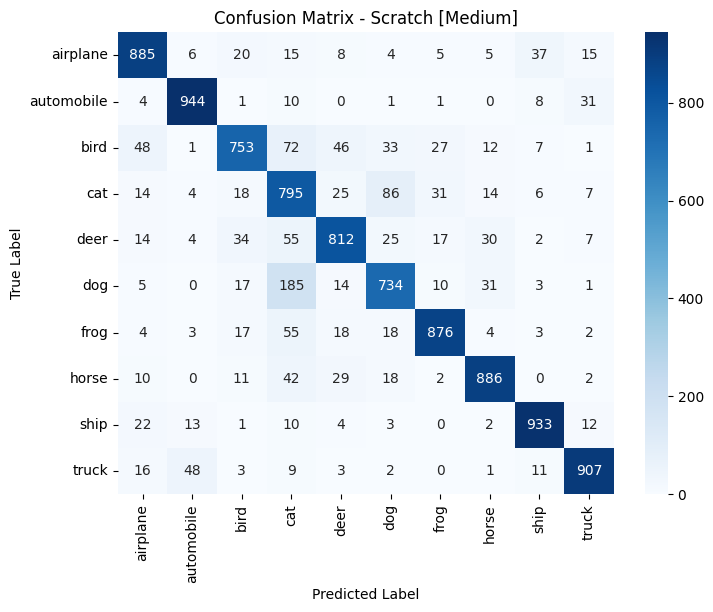
\includegraphics[width=0.45\textwidth]{confusion_matrix_scratch05_complex}
        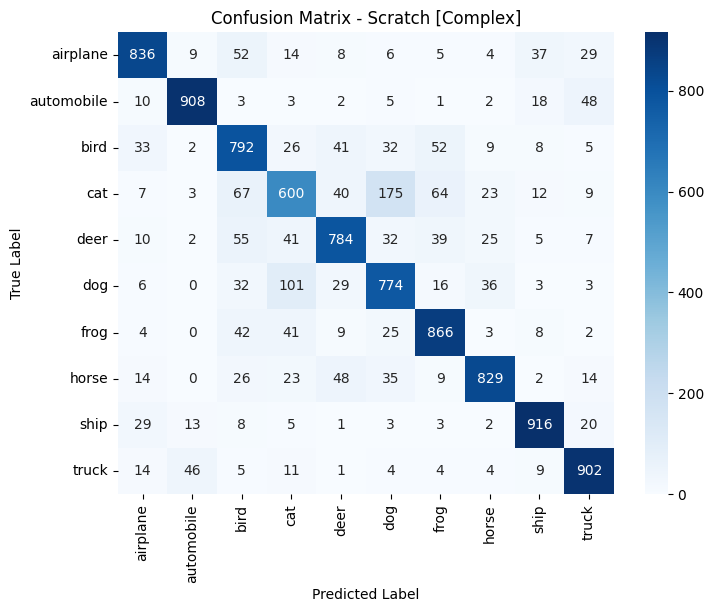
\includegraphics[width=0.45\textwidth]{confusion_matrix_scratch06}
        \label{fig:confussion_matrix_scratach}
    \end{figure}

    The conclusions of this part are:
    \begin{enumerate}
        \item Approximately 60 epochs should be sufficient to reach 90\% accuracy.
        \item With just images of 32x32 it can be possible to reach 80\% accuracy.
        \item As the image size increases, the model's complexity should also increase.
        \item Since the algorithm learns quickly during the initial epochs, implementing a learning rate schedule or decay would be beneficial.
    \end{enumerate}

    \large\textbf{Part II: Transfer learning for image classification}

    \begin{enumerate}
        \item \textbf{MobileNet}: As suggested, I started with this architecture, which gave me a glimpse of how easy it is to apply transfer learning.
        \begin{enumerate}
            \item \textbf{With a size of 224x224}: The first iteration was run using only the CPU, and each epoch took 25 minutes.
            Surprisingly, it easily matched the performance of the model I had trained from scratch.
            The key aspect of this iteration was that I resized the images to 224x224 and used the following optimizer:
            \lstinline|optim.SGD(model.parameters(), lr=0.001, momentum=0.9)|.
            To my surprise, the model got stuck after a few epochs, so I decided to tweak the hyperparameters.

            \item \textbf{With a size of 64x64}: The next iteration used a GPU, reducing the training time per epoch to 3 minutes.
            I noticed that the GPU was not fully utilized, so I increased the batch size to 256.
            Additionally, increasing the learning rate allowed for a more complex classification layer.

            \begin{enumerate}
                \item \textbf{First 30 epochs}: Only the last classification layer was unfrozen, meaning all pre-trained layers remained frozen.
                \item \textbf{Last 30 epochs}: All layers were unfrozen.
                The transition was performed manually in a Jupyter notebook cell, so the code used for this transition is not included here.
            \end{enumerate}

            \item This transition improved performance and accelerated training over the epochs.
        \end{enumerate}

        \item \textbf{ResNet}: This architecture comes in different levels of complexity.
        In this case, I used \href{https://pytorch.org/tutorials/beginner/transfer_learning_tutorial.html}{ResNet18 from the tutorial} and ResNet50 from the official documentation.

        \begin{enumerate}
            \item \textbf{ResNet18 - Fine-tuning (Tutorial Part 1)}:
            The tutorial suggests that this model is intended for small datasets.
            This might explain why the model got stuck after the initial epochs.

            \item \textbf{ResNet18 - Feature Extractor (Tutorial Part 2)}:
            Freezing all layers except the last one worsened the learning process.
            This was not surprising, given the behavior I had observed in the previous experiment.
            In both tutorial parts, images of size 224x224 were used.

            \item \textbf{ResNet50}: After experimenting with simpler models, I switched to ResNet50,
            applying the same strategy—freezing all layers except the last ones and later unfreezing them.

            \begin{enumerate}
                \item \textbf{First 30 epochs}: Only three residual blocks were unfrozen:
                \begin{lstlisting}
for param in model.parameters():
    param.requires_grad = False

for param in model.layer4.parameters():
    param.requires_grad = True

for param in model.fc.parameters():
    param.requires_grad = True
                \end{lstlisting}

                \item \textbf{Last 30 epochs}: All layers were unfrozen.
                The transition was performed manually in a Jupyter notebook cell, so the code used for this transition might not be consistent in the final script.

                \item Again, this transition improved the model's performance.
            \end{enumerate}
        \end{enumerate}

        \item \textbf{EfficientNet}:
        According to the documentation, this model is designed for small images, so I did not resize the original images.
        Unfortunately, with the hyperparameters I used, it performed worse than the other models.
        Additionally, my GPU quota was exhausted, so I could not run further iterations.
    \end{enumerate}

    \begin{figure}[h]
        \caption{Train and Validation / Loss and Accuracy}
        \centering
        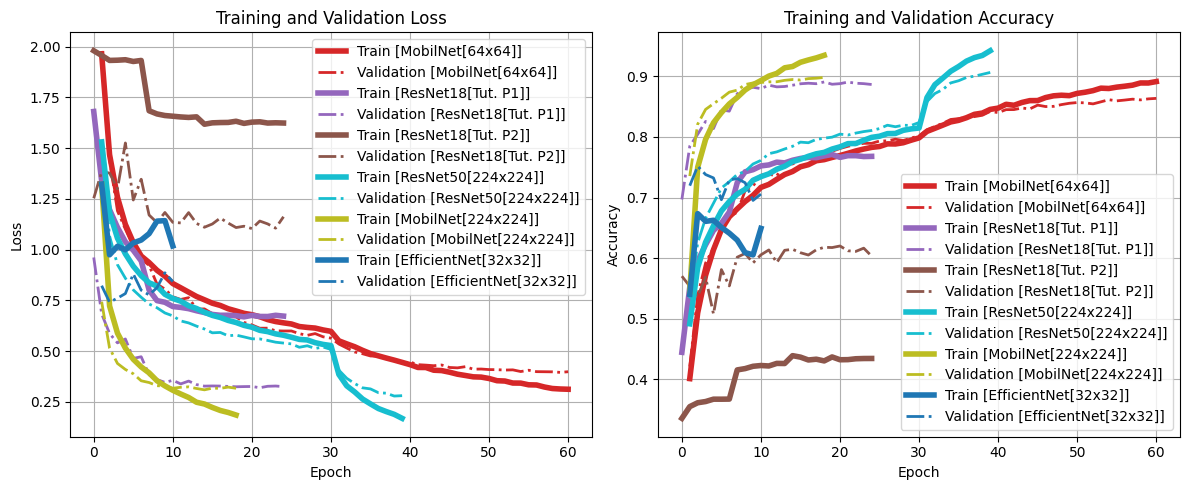
\includegraphics[width=0.9\textwidth]{training_metrics_pretrained_01}
        \label{fig:training_metrics_pretrained_01}
    \end{figure}
    \begin{figure}[h]
        \caption{Confussion Matrix for pre-trained models}
        \centering
        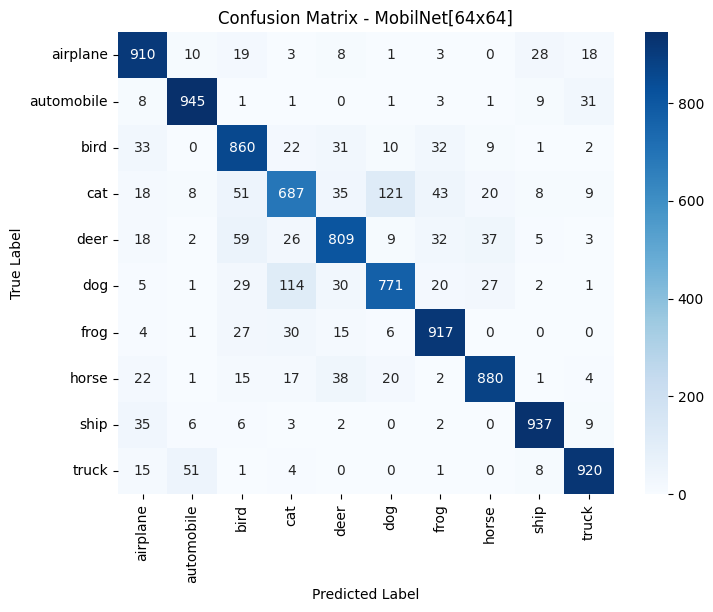
\includegraphics[width=0.3\textwidth]{confusion_matrix_mobilnet64}
        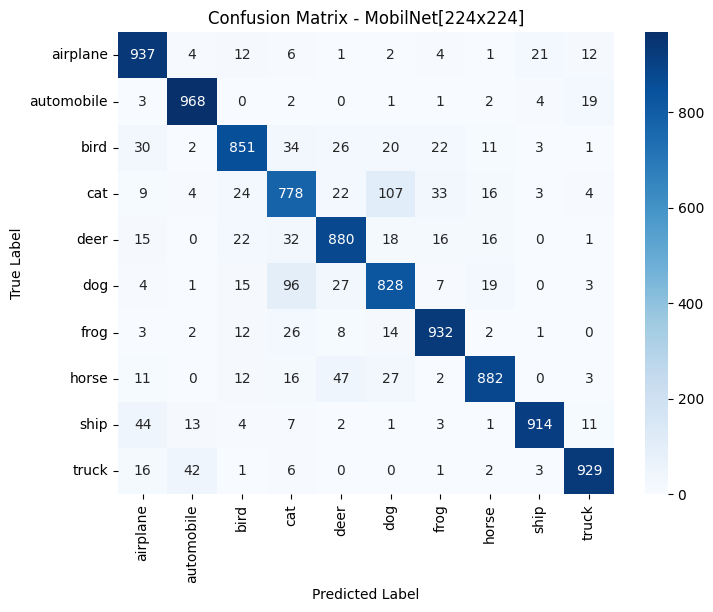
\includegraphics[width=0.3\textwidth]{confusion_matrix_mobilnet224}
        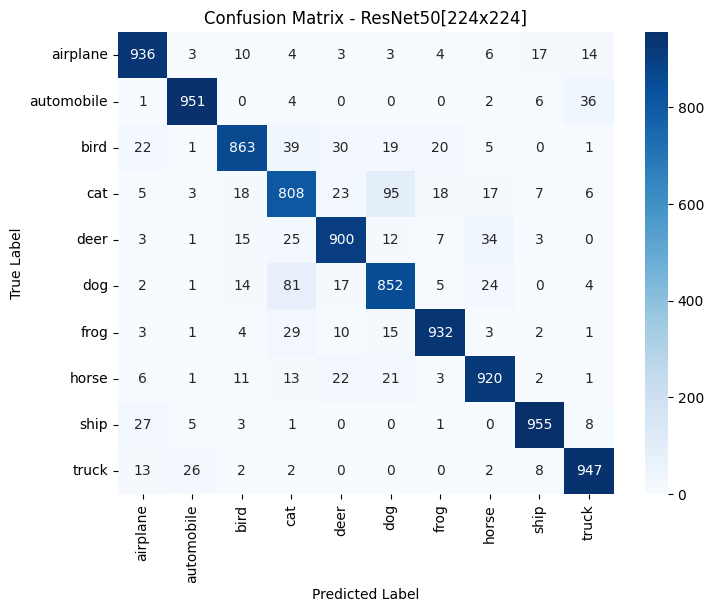
\includegraphics[width=0.3\textwidth]{confusion_matrix_resnet50}
        \label{fig:confussion_matrix_pretrained}
    \end{figure}

    The conclusions of this part are:
    \begin{enumerate}
        \item MobilNet performed well even for small and bigger images.
        \item Resnet50 performed better, that was expected since it is a complex model.
        \item The strategy of freezing almost all layers then unfreezing them after some epochs worked pretty well.
    \end{enumerate}

    \large\textbf{Part III: Prediction}
    Among all models three of them perform quite similar, MobilNet64x64, MobilNet224x224 and Resnet50.
    For practice purposes I've decided to use them at once to make the prediction or final model.
    The strategy to follow is by vote, if there is a tie (all of them indicates different classifications) the Resnet50 is preferred.

    The idea is as follows: \lstinline|predict_only_labels| returns the file names (for further ordering) and the predictions of the label.
    Then I apply the vote with the following code:
    \begin{lstlisting}
def predict_by_quorum_only_labels(models_with_loaders):
    predictions = [(predict_only_labels(model_iteration, model_loader), weight) for model_iteration, model_loader, weight in models_with_loaders]
    final_predictions = []
    for ((a, b), c) in zip(zip(predictions[0][0][1], predictions[1][0][1]), predictions[2][0][1]):
        if a == b or b == c:
            final_predictions.append(b)
        elif a == c:
            final_predictions.append(a)
        else:
            final_predictions.append(b)
    final_predictions = np.array(final_predictions)
    return predictions[0][0][0], final_predictions

    \end{lstlisting}

    The result of this approach can be shown in the next table, when all three of them participant the accuracy reaches to 91.88\%.
    The confusion matrix also is improved, I will show it side to side against ResNet50. \\

    \begin{center}

\begin{tabular}{||l | r||}
 \hline
 Model & Accuracy \\ [0.5ex]
 \hline\hline
 MobilNet[64x64] & 86.36\% \\ \hline
 MobilNet[224x224] & 89.82\% \\ \hline
 ResNet50[224x224] & 90.64\% \\
 \hline \hline
 All three of them by vote & 91.88\% \\ [1ex]
 \hline
\end{tabular}
\end{center}

    \begin{figure}[h]
        \caption{Confussion Matrix comparing ResNet50[224x224] vs (MobilNet 64x64, MobilNet 224x224, Resnet50 224x224)}
        \centering
        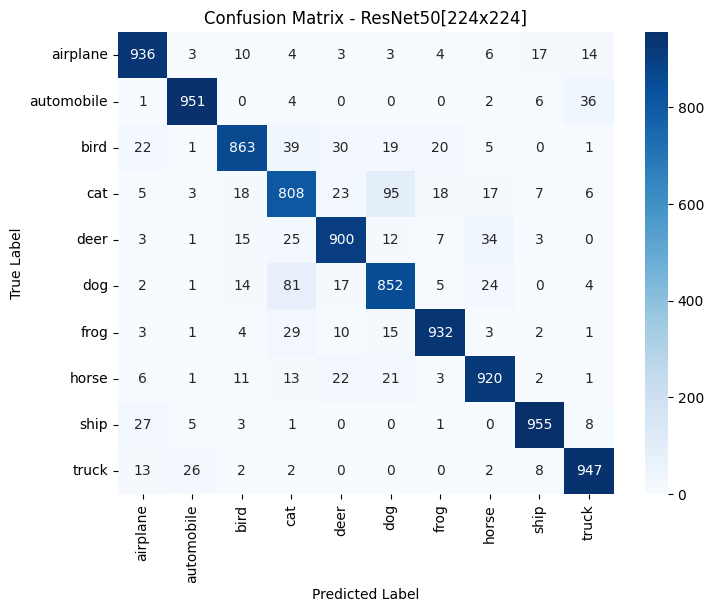
\includegraphics[width=0.45\textwidth]{confusion_matrix_resnet50}
        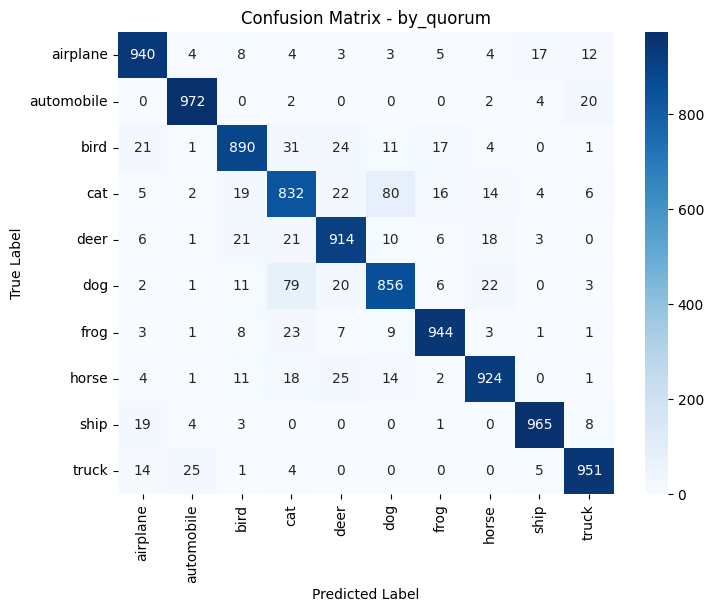
\includegraphics[width=0.45\textwidth]{confusion_matrix_by_quorum}
        \label{fig:confussion_matrix_quorum}
    \end{figure}

    With that final predictor I completed the predictions of unlabelled images.

    \large\textbf{Extra}
    All code used for experiments mentioned, and the scripts to generate this report are in \href{https://github.com/vmchura/practice_pytorch_images}{this repository of GitHub https://github.com/vmchura/practice\_pytorch\_images}.

\end{document}